%\clearpage
\section{Background Estimation Techniques}
\label{sec:bkg}

In this section we describe the techniques used to estimate the SM backgrounds in our signal regions defined by requirements of large \MET.
The SM backgrounds fall into three categories:

\begin{itemize}
\item \zjets: this is the dominant background after the preselection. The \MET\ in \zjets\ events is estimated with the 
``\MET\ templates'' technique described in Sec.~\ref{sec:bkg_zjets};
\item Flavor-symmetric (FS) backgrounds: this category includes processes which produces 2 leptons of uncorrelated flavor. It is dominated
by \ttbar\ but also contains Z$\to\tau\tau$, WW, and single top processes. This is the dominant contribution in the signal regions, and it
is estimated using a data control sample of e$\mu$ events as described in Sec.~\ref{sec:bkg_fs};
\item WZ and ZZ backgrounds: this background is estimated from MC, after validating the MC modeling of these processes using data control
samples with jets and exactly 3 leptons (WZ control sample) and exactly 4 leptons (ZZ control sample) as described in Sec.~\ref{sec:bkg_vz};
%\item Rare SM backgrounds: this background contains rare processes such as $t\bar{t}$V and triple vector boson processes VVV (V=W,Z).
%This background is estimated from MC as described in Sec.~\ref{sec:bkg_raresm}. {\bf FIXME: add rare MC}
\end{itemize}

\subsection{Estimating the \zjets\ Background with \MET\ Templates}
\label{sec:bkg_zjets}

The premise of this data driven technique is that \MET\ in \zjets\ events
is produced by the hadronic recoil system and {\it not} by the leptons making up the Z.
Therefore, the basic idea of the \MET\ template method is to measure the \MET\ distribution in 
a control sample which has no true MET and the same general attributes regarding
fake MET as in \zjets\ events. We thus use a sample of \gjets\ events, since both \zjets\
and \gjets\ events consist of a well-measured object recoiling against hadronic jets.

For selecting photon-like objects, the very loose photon selection described in Sec.~\ref{sec:phosel} is used.
It is not essential for the photon sample to have high purity. For our purposes, selecting jets with predominantly 
electromagnetic energy deposition in a good fiducial volume suffices to ensure that 
they are well measured and do not contribute to fake \MET. The \gjets\ events are selected with a suite of
single photon triggers with \pt thresholds varying from 22--90 GeV. The events are weighted by the trigger prescale
such that \gjets\ events evenly sample the conditions over the full period of data taking.
There remains a small difference in the PU conditions in the \gjets\ vs. \zjets\ samples due to the different
dependencies of the $\gamma$ vs. Z isolation efficiencies on PU. To account for this, we reweight the \gjets\ samples
to match the distribution of reconstructed primary vertices in the \zjets\ sample.

To account for kinematic differences between the hadronic systems in the control vs. signal 
samples, we measure the \MET\ distributions in the \gjets\ sample in bins of the number of jets 
and the scalar sum of jet transverse energies (\Ht). These \MET\ templates are extracted separately from the 5 single photon
triggers with thresholds 22, 36, 50, 75, and 90 GeV, so that the templates are effectively binned in photon \pt.
All \MET distributions are normalized to unit area to form ``MET templates''.
The prediction of the MET in each \Z event is the template which corresponds to the \njets,
\Ht, and Z \pt in the \zjets\ event. The prediction for the \Z sample is simply the sum of all such templates.
All templates are displayed in App.~\ref{app:templates}.

After preselection, there is  a small contribution from backgrounds other than \zjets. To correct for this, the \MET\ templates
prediction is scaled such that the total background prediction matches the observed data yield in the \MET\ 0--60 GeV region.
Because the non-\zjets impurity in the low \MET\ region after preselection is very small, this results in 
scaling factors of 0.985 (0.995) for the inclusive (targeted) search.

\subsection{Estimating the Flavor-Symmetric Background with e$\mu$ Events}
\label{sec:bkg_fs}

In this subsection we describe the background estimate for the FS background. Since this background produces equal rates of same-flavor (SF)
ee and $\mu\mu$ lepton pairs as opposite-flavor (OF) e$\mu$ lepton pairs, the OF yield can be used to estimate the SF yield, after
correcting for the different electron vs. muon offline selection efficiencies and the different efficiencies for the ee, $\mu\mu$, and e$\mu$ triggers.

An important quantity needed to translate from the OF yield to a prediction for the background in the SF final state is the ratio 
$R_{\mu e} = \epsilon_\mu / \epsilon_e$, where $\epsilon_\mu$ ($\epsilon_e$) indicates the offline muon (electron) selection efficiency. 
This quantity can be extracted from data using the observed Z$\to\mu\mu$ and Z$\to$ee yields in the preselection region, after correcting 
for the different trigger efficiencies.

Hence we define:

\begin{itemize}
\item $N_{ee}^{\rm{trig}} = \epsilon_{ee}^{\rm{trig}}N_{ee}^{\rm{offline}}$,
\item $N_{\mu\mu}^{\rm{trig}} = \epsilon_{\mu\mu}^{\rm{trig}}N_{\mu\mu}^{\rm{offline}}$,
\item $N_{e\mu}^{\rm{trig}} = \epsilon_{e\mu}^{\rm{trig}}N_{e\mu}^{\rm{offline}}$.
\end{itemize}
 
Here $N_{\ell\ell}^{\rm{trig}}$ denotes the number of selected Z events in the $\ell\ell$ channel passing the offline and trigger selection
(in other words, the number of recorded and selected events), $\epsilon_{\ell\ell}^{\rm{trig}}$ is the trigger efficiency, and 
$N_{\ell\ell}^{\rm{offline}}$ is the number of events that would have passed the offline selection if the trigger had an efficiency of 100\%.
Thus we calculate the quantity:

\begin{equation}
R_{\mu e} = \sqrt{\frac{N_{\mu\mu}^{\rm{offline}}}{N_{ee}^{\rm{offline}}}} = \sqrt{\frac{N_{\mu\mu}^{\rm{trig}}/\epsilon_{\mu\mu}^{\rm{trig}}}{N_{ee}^{\rm{trig}}/\epsilon_{ee}^{\rm{trig}}}} 
= \sqrt{\frac{304953/0.88}{239661/0.95}} = 1.17\pm0.07.
\end{equation}

Here we have used the Z$\to\mu\mu$ and Z$\to$ee yields from Table~\ref{table:zyields_2j} and the trigger efficiencies quoted in Sec.~\ref{sec:datasets}.
The indicated uncertainty is due to the 3\% uncertainties in the trigger efficiencies. %{\bf FIXME: check for variation w.r.t. lepton \pt}.
The predicted yields in the ee and $\mu\mu$ final states are calculated from the observed e$\mu$ yield as

\begin{itemize}
\item $N_{ee}^{\rm{predicted}}    = \frac {N_{e\mu}^{\rm{trig}}} {\epsilon_{e\mu}^{\rm{trig}}} \frac {\epsilon_{ee}^{\rm{trig}}} {2 R_{\mu e}} 
= \frac{N_{e\mu}^{\rm{trig}}}{0.92}\frac{0.95}{2\times1.17} = (0.44\pm0.05) \times N_{e\mu}^{\rm{trig}}$ ,
\item $N_{\mu\mu}^{\rm{predicted}} = \frac {N_{e\mu}^{\rm{trig}}} {\epsilon_{e\mu}^{\rm{trig}}} \frac {\epsilon_{\mu\mu}^{\rm{trig}} R_{\mu e}}  {2}
= \frac {N_{e\mu}^{\rm{trig}}} {0.95} \frac {0.88 \times 1.17}{2} = (0.54\pm0.07) \times N_{e\mu}^{\rm{trig}}$,
\end{itemize}

and the predicted yield in the combined ee and $\mu\mu$ channel is simply the sum of these two predictions:

\begin{itemize}
\item $N_{ee+\mu\mu}^{\rm{predicted}} = (0.98\pm0.06)\times N_{e\mu}^{\rm{trig}}$.
\end{itemize}

Note that the relative uncertainty in the combined ee and $\mu\mu$ prediction is smaller than those for the individual ee and $\mu\mu$ predictions
because the uncertainty in $R_{\mu e}$ cancels when summing the ee and $\mu\mu$ predictions. %{\bf N.B. these uncertainties are preliminary}.

To improve the statistical precision of the FS background estimate, we remove the requirement that the e$\mu$ lepton pair falls in the Z mass window.
Instead we scale the e$\mu$ yield by $K$, the efficiency for e$\mu$ events to satisfy the Z mass requirement, extracted from simulation. In Fig.~\ref{fig:K_incl}
we display the value of $K$ in data and simulation, for a variety of \MET\ requirements, for the inclusive analysis. 
Based on this we chose $K=0.14\pm0.02$ for the lower \MET\ regions, $K=0.14\pm0.04$ for the \MET\ $>$ 200 GeV region,and $K=0.14\pm0.09$ for \MET\ $>$ 300 GeV,
where the larger uncertainties reflect the reduced statistical precision at large \MET.
The corresponding plot for the targeted analysis, including the b-veto, is displayed in Fig.~\ref{fig:K_targeted}.
Based on this we chose $K=0.13\pm0.02$
for all \MET\ regions up to  \MET\ $>$ 150 GeV. For the \MET\ $>$ 200 GeV region we choose $K=0.13\pm0.05$, due to the reduced  statistical precision.

\begin{figure}[!ht]
\begin{center}
\begin{tabular}{cc}
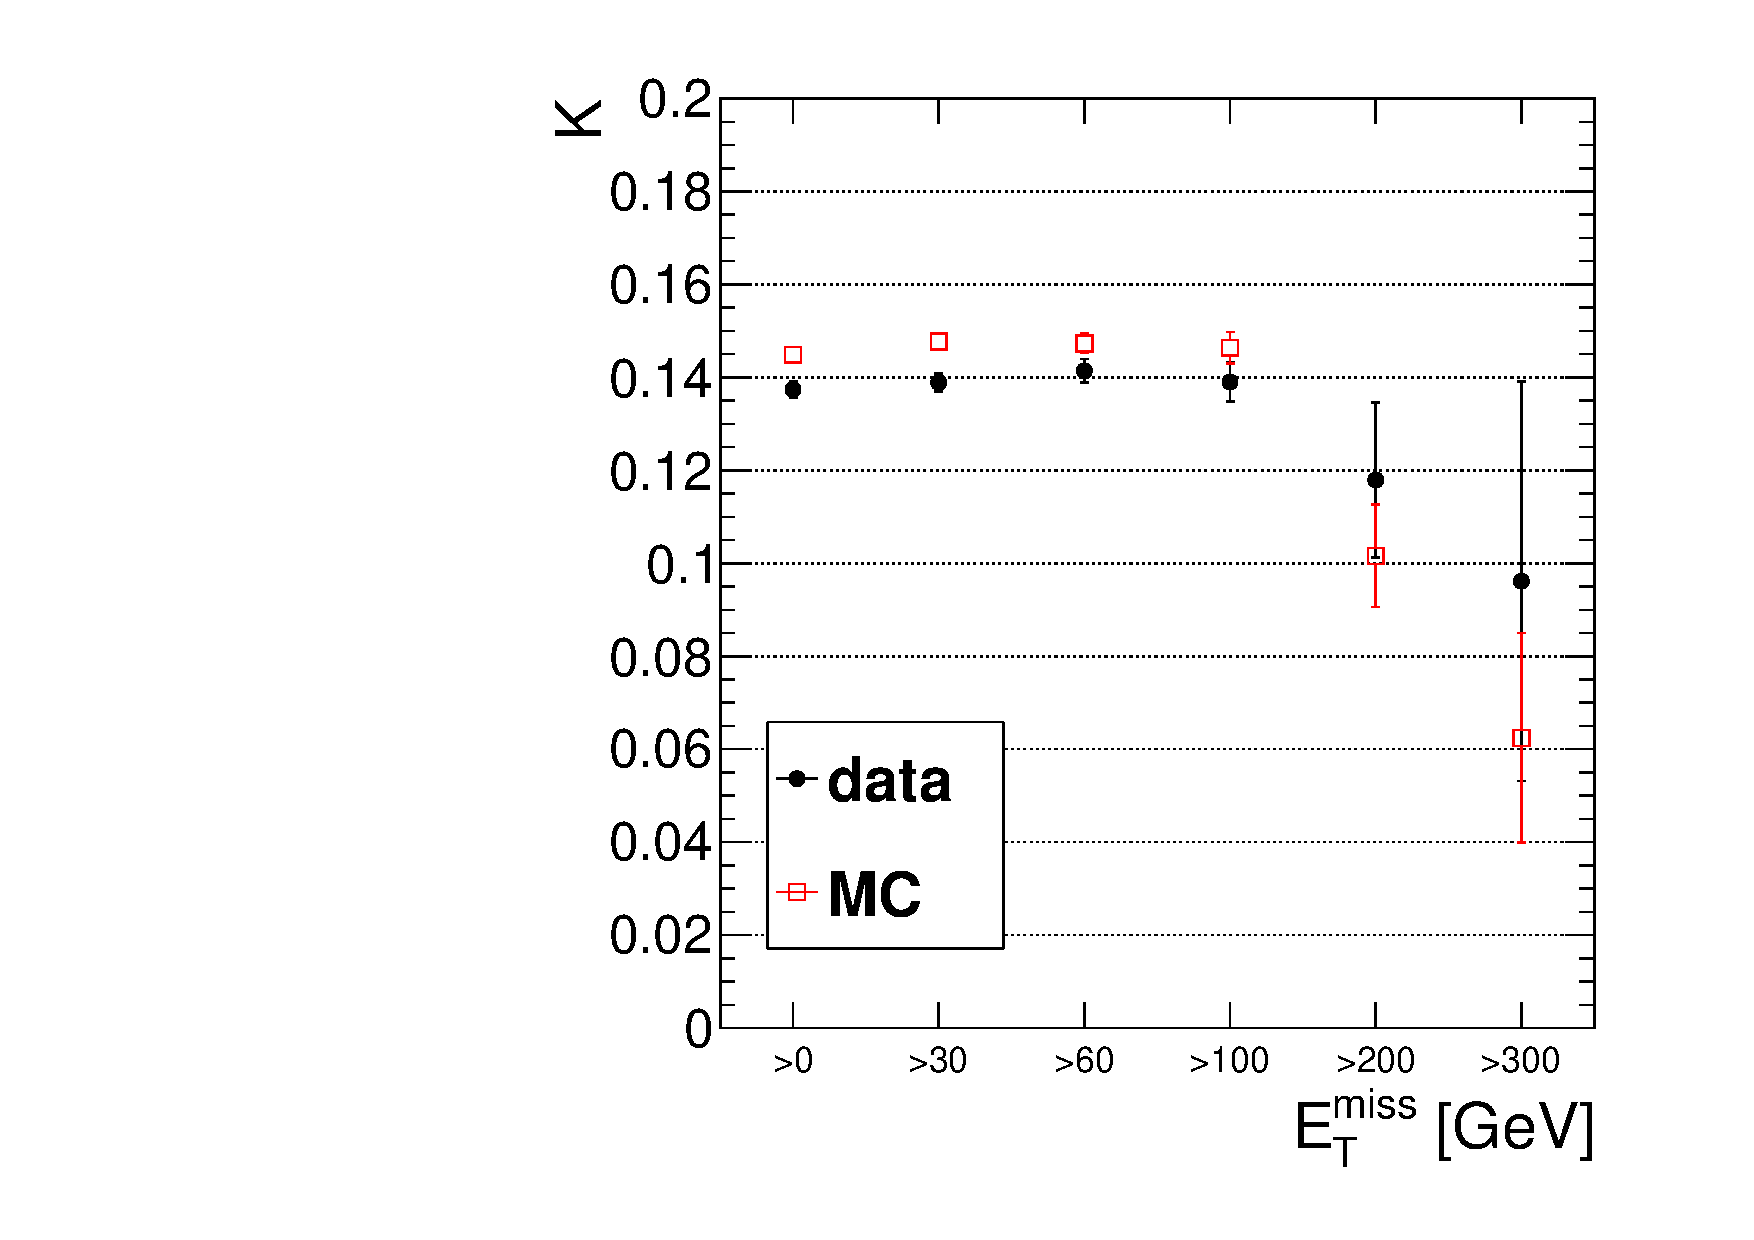
\includegraphics[width=0.4\textwidth]{plots/extractK_inclusive_19p5fb.pdf} &
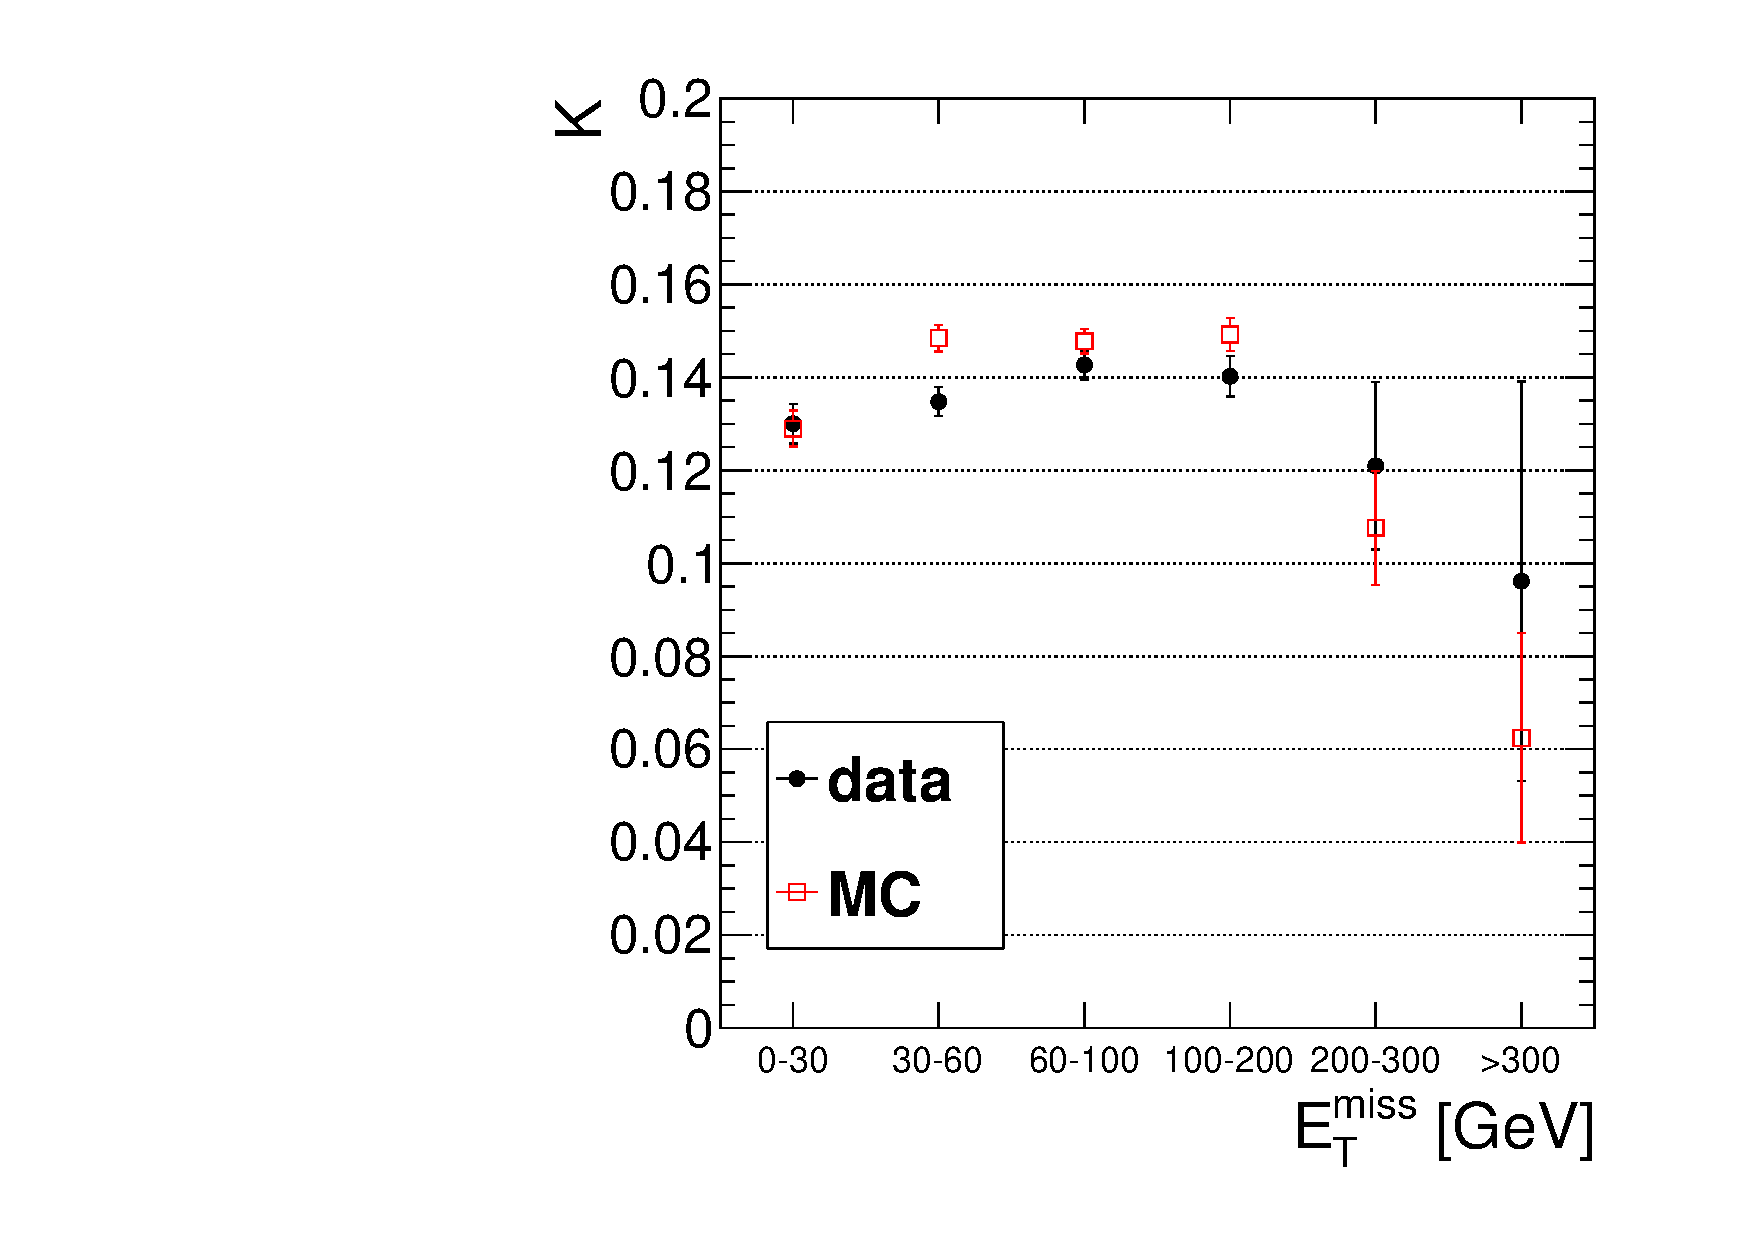
\includegraphics[width=0.4\textwidth]{plots/extractK_exclusive_19p5fb.pdf} \\
\end{tabular}
\caption{\label{fig:K_incl}
The efficiency for e$\mu$ events to satisfy the dilepton mass requirement, $K$, in data and simulation for inclusive \MET\ intervals (left) and
exclusive \MET\ intervals (right) for the inclusive analysis. 
}

\begin{comment}

Using selection : ((((leptype==2)&&(csc==0 && hbhe==1 && hcallaser==1 && ecaltp==1 && trkfail==1 && eebadsc==1 && hbhenew==1))&&(isdata==0 || (run<197556 || run>198913)))&&(njets>=2))&&(lep1.pt()>20 && lep2.pt()>20)
Using weight    : vtxweight * weight
OF entries (total)  43808
OF entries (Z mass) 6021
K                   0.137441
Info in <TCanvas::MakeDefCanvas>:  created default TCanvas with name c1

--------------------------------------------------------------
pfmet>0

data  : 
total : 43808
Z     : 6021
K     : 0.14 +/- 0.002

MC    : 
total : 2378.42
Z     : 344.559
K     : 0.14 +/- 0.002
--------------------------------------------------------------


--------------------------------------------------------------
pfmet>30

data  : 
total : 36603
Z     : 5084
K     : 0.14 +/- 0.002

MC    : 
total : 2012.6
Z     : 297.342
K     : 0.15 +/- 0.002
--------------------------------------------------------------


--------------------------------------------------------------
pfmet>60

data  : 
total : 22692
Z     : 3209
K     : 0.14 +/- 0.002

MC    : 
total : 1285.07
Z     : 189.292
K     : 0.15 +/- 0.002
--------------------------------------------------------------


--------------------------------------------------------------
pfmet>100

data  : 
total : 7862
Z     : 1093
K     : 0.14 +/- 0.004

MC    : 
total : 470.932
Z     : 68.9364
K     : 0.15 +/- 0.003
--------------------------------------------------------------


--------------------------------------------------------------
pfmet>200

data  : 
total : 424
Z     : 50
K     : 0.12 +/- 0.017

MC    : 
total : 28.2757
Z     : 2.87288
K     : 0.10 +/- 0.011
--------------------------------------------------------------


--------------------------------------------------------------
pfmet>300

data  : 
total : 52
Z     : 5
K     : 0.10 +/- 0.043

MC    : 
total : 3.77378
Z     : 0.235632
K     : 0.06 +/- 0.023
--------------------------------------------------------------

Using selection : ((((leptype==2)&&(csc==0 && hbhe==1 && hcallaser==1 && ecaltp==1 && trkfail==1 && eebadsc==1 && hbhenew==1))&&(isdata==0 || (run<197556 || run>198913)))&&(njets>=2))&&(lep1.pt()>20 && lep2.pt()>20)
Using weight    : vtxweight * weight
OF entries (total)  43808
OF entries (Z mass) 6021
K                   0.137441
Warning in <TROOT::Append>: Replacing existing TH1: htot (Potential memory leak).
Warning in <TROOT::Append>: Replacing existing TH1: hZ (Potential memory leak).

--------------------------------------------------------------
pfmet>0   && pfmet<30

data  : 
total : 7205
Z     : 937
K     : 0.13 +/- 0.004

MC    : 
total : 366.332
Z     : 47.2379
K     : 0.13 +/- 0.004
--------------------------------------------------------------


--------------------------------------------------------------
pfmet>30  && pfmet<60

data  : 
total : 13911
Z     : 1875
K     : 0.13 +/- 0.003

MC    : 
total : 727.951
Z     : 108.068
K     : 0.15 +/- 0.003
--------------------------------------------------------------


--------------------------------------------------------------
pfmet>60  && pfmet<100

data  : 
total : 14830
Z     : 2116
K     : 0.14 +/- 0.003

MC    : 
total : 814.344
Z     : 120.355
K     : 0.15 +/- 0.003
--------------------------------------------------------------


--------------------------------------------------------------
pfmet>100 && pfmet<200

data  : 
total : 7438
Z     : 1043
K     : 0.14 +/- 0.004

MC    : 
total : 442.657
Z     : 66.0631
K     : 0.15 +/- 0.004
--------------------------------------------------------------


--------------------------------------------------------------
pfmet>200 && pfmet<300

data  : 
total : 372
Z     : 45
K     : 0.12 +/- 0.018

MC    : 
total : 24.502
Z     : 2.63725
K     : 0.11 +/- 0.012
--------------------------------------------------------------


--------------------------------------------------------------
pfmet>300

data  : 
total : 52
Z     : 5
K     : 0.10 +/- 0.043

MC    : 
total : 3.77378
Z     : 0.235632
K     : 0.06 +/- 0.023
--------------------------------------------------------------


\end{comment}

\end{center}
\end{figure}

\begin{figure}[!hb]
\begin{center}
\begin{tabular}{cc}
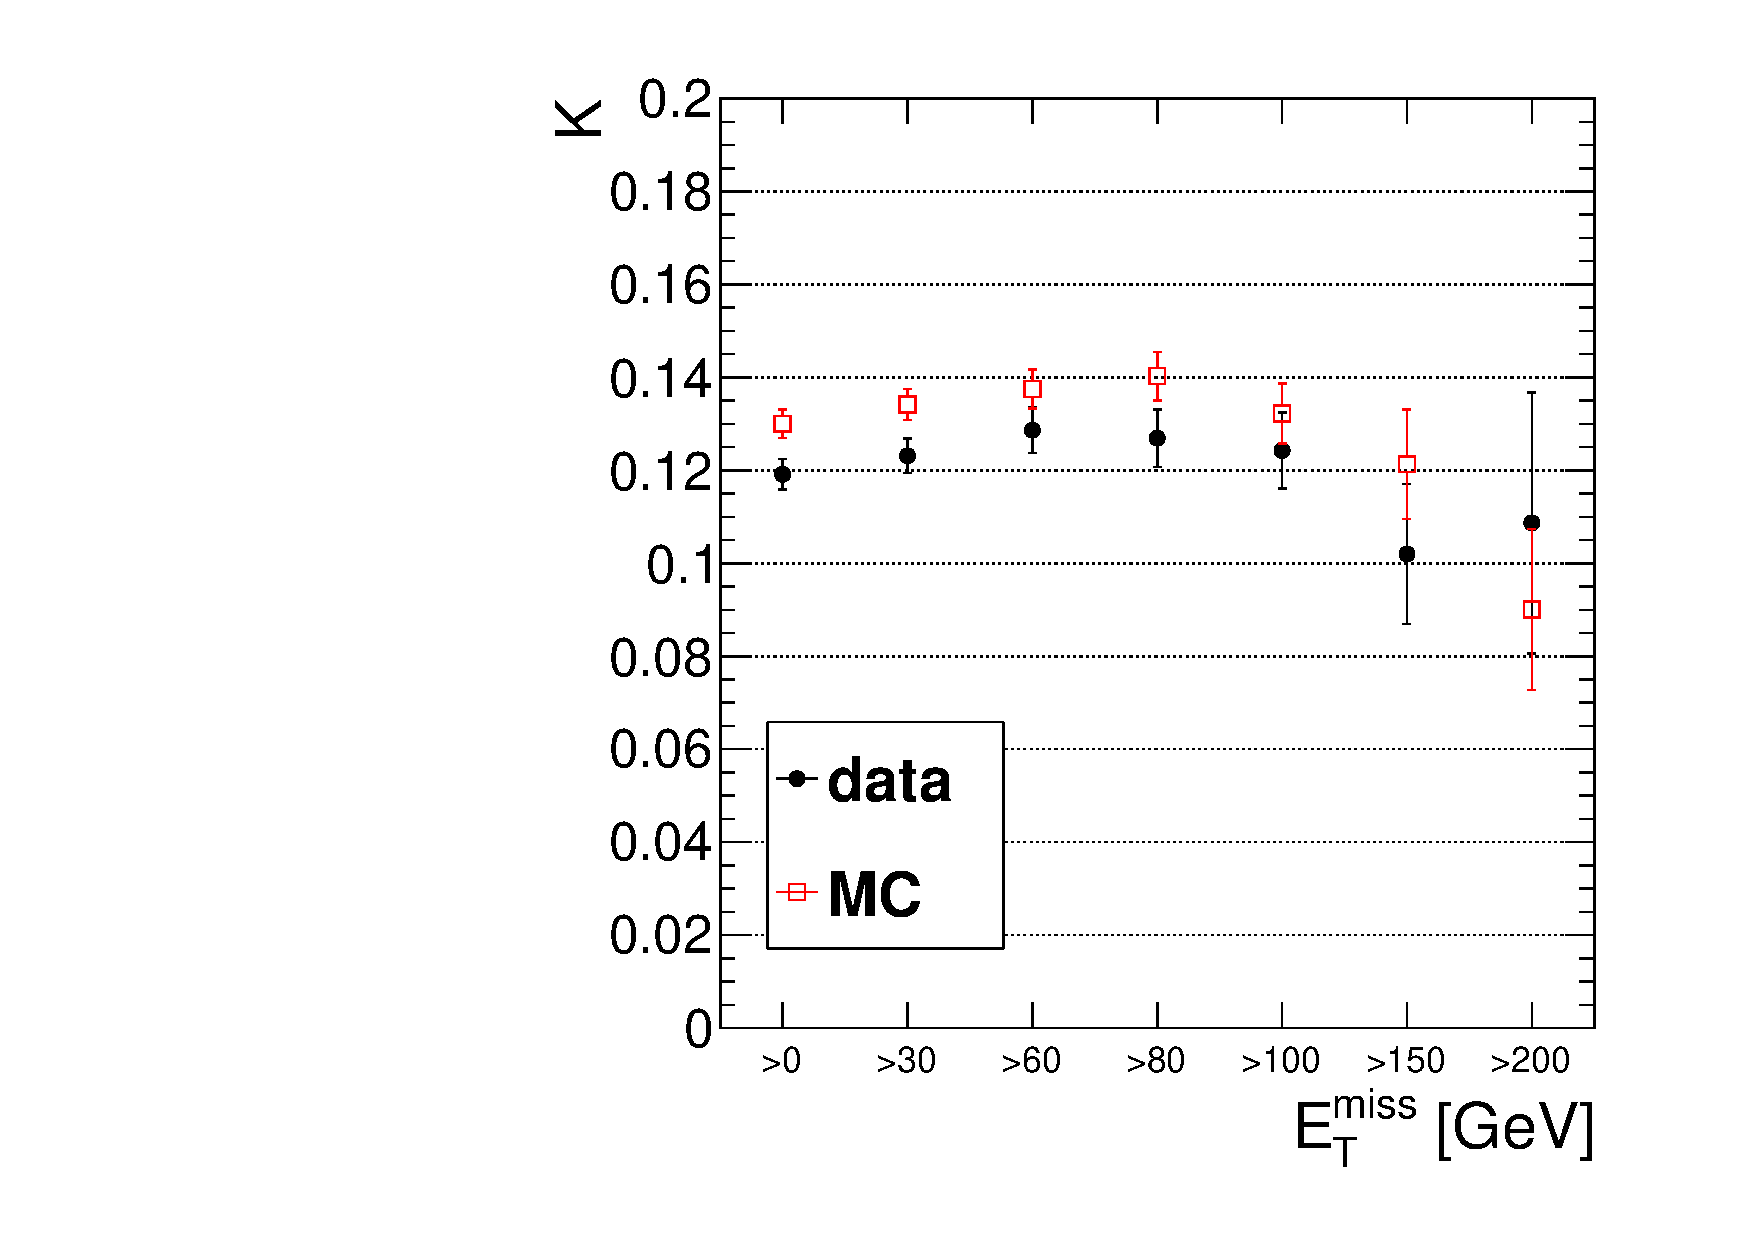
\includegraphics[width=0.4\textwidth]{plots/extractK_inclusive_bveto_19p5fb.pdf} &
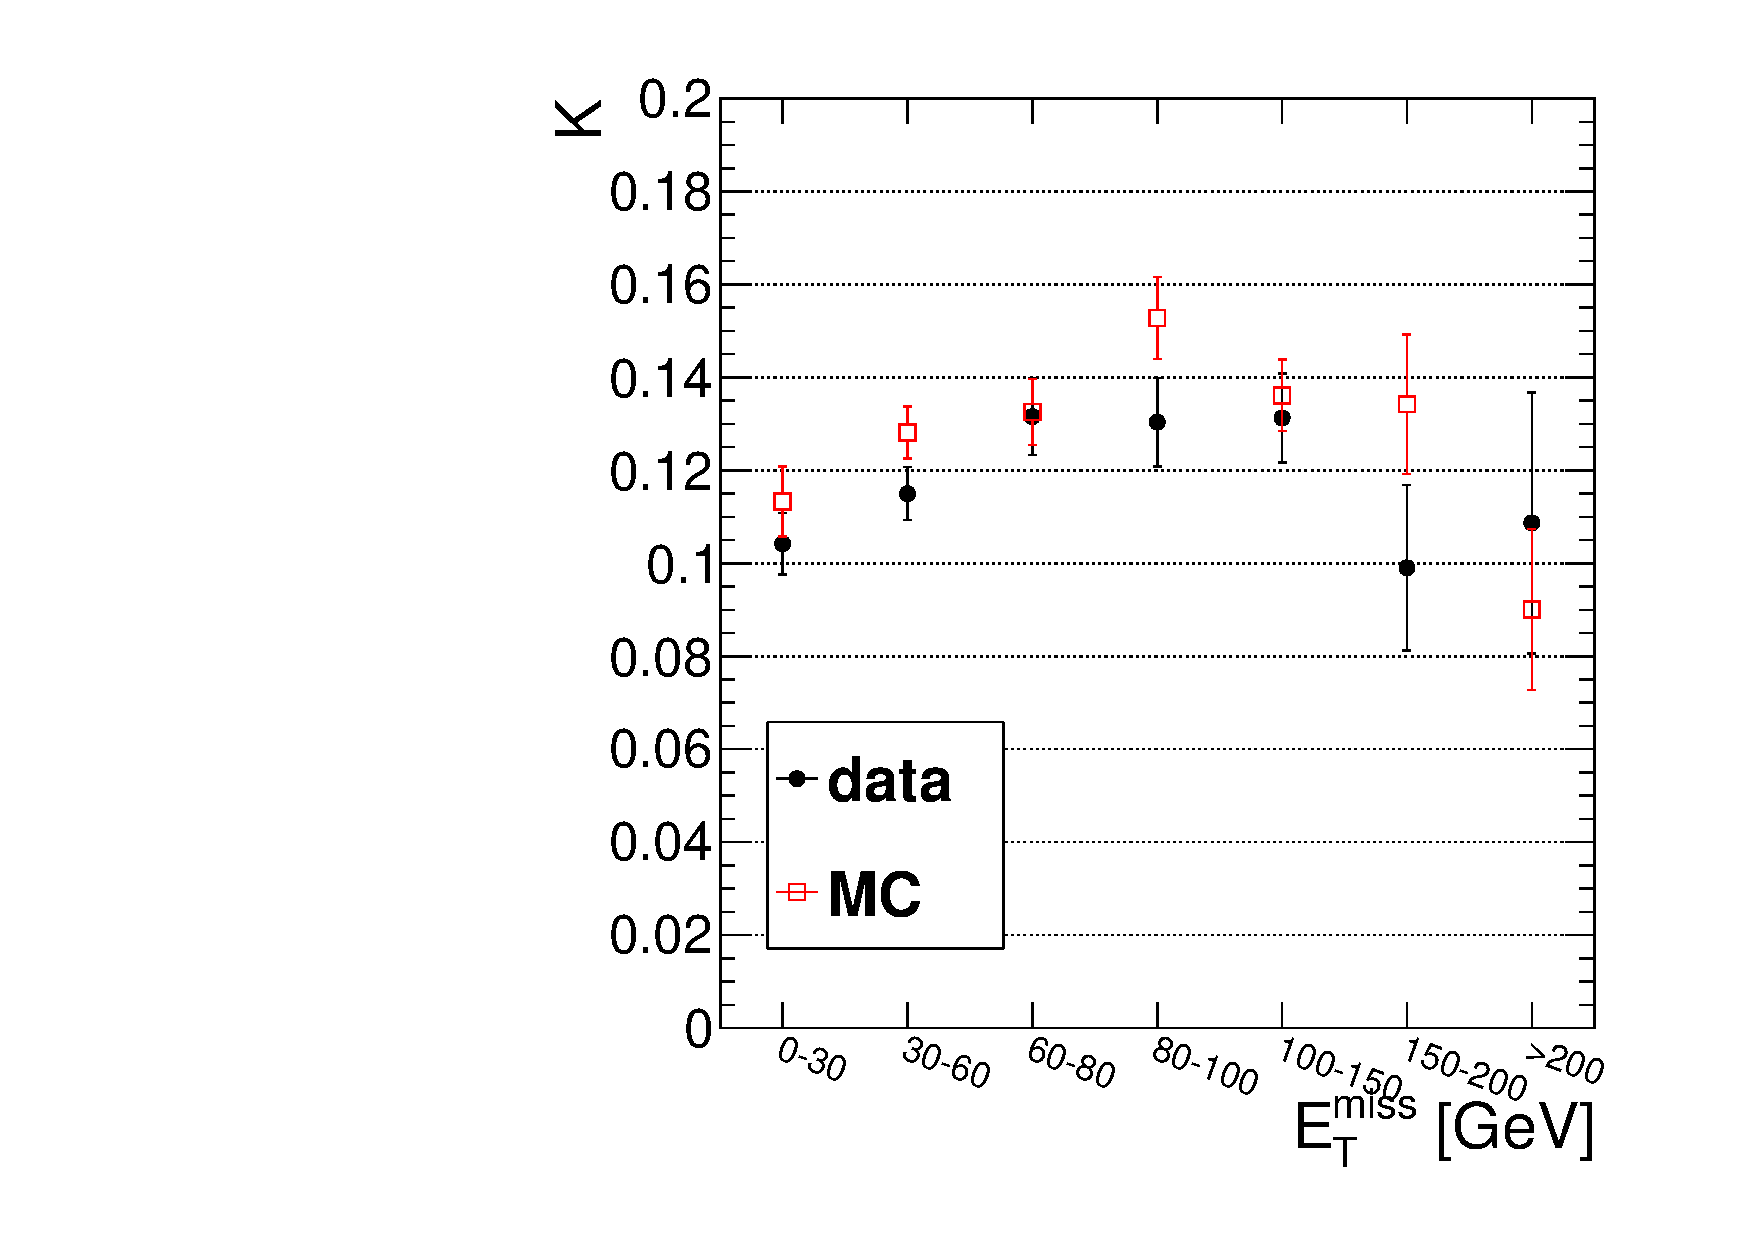
\includegraphics[width=0.4\textwidth]{plots/extractK_exclusive_bveto_19p5fb.pdf} \\
\end{tabular}
\caption{
The efficiency for e$\mu$ events to satisfy the dilepton mass requirement, $K$, in data and simulation for inclusive \MET\ intervals (left) and
exclusive \MET\ intervals (right) for the targeted analysis, including the b-veto. 
Based on this we chose $K=0.13\pm0.02$ for the \MET\ regions up to \MET\ $>$ 100 GeV.
For higher \MET\ regions we chose $K=0.13\pm0.07$.
%{\bf FIXME plots made with 10\% of \zjets\ MC statistics, to be remade with full statistics}
\label{fig:K_targeted}
}
\begin{comment}

Using selection : (((((leptype==2)&&(csc==0 && hbhe==1 && hcallaser==1 && ecaltp==1 && trkfail==1 && eebadsc==1 && hbhenew==1))&&(isdata==0 || (run<197556 || run>198913)))&&(njets>=2))&&(lep1.pt()>20 && lep2.pt()>20))&&(nbcsvm==0)
Using weight    : vtxweight * weight
OF entries (total)  11172
OF entries (Z mass) 1331
K                   0.119137
Info in <TCanvas::MakeDefCanvas>:  created default TCanvas with name c1

--------------------------------------------------------------
pfmet>0

data  : 
total : 11172
Z     : 1331
K     : 0.12 +/- 0.003

MC    : 
total : 556.3
Z     : 72.3357
K     : 0.13 +/- 0.003
--------------------------------------------------------------


--------------------------------------------------------------
pfmet>30

data  : 
total : 8811
Z     : 1085
K     : 0.12 +/- 0.004

MC    : 
total : 447.641
Z     : 60.0542
K     : 0.13 +/- 0.003
--------------------------------------------------------------


--------------------------------------------------------------
pfmet>60

data  : 
total : 5263
Z     : 677
K     : 0.13 +/- 0.005

MC    : 
total : 285.463
Z     : 39.2608
K     : 0.14 +/- 0.004
--------------------------------------------------------------


--------------------------------------------------------------
pfmet>80

data  : 
total : 3325
Z     : 422
K     : 0.13 +/- 0.006

MC    : 
total : 183.689
Z     : 25.7671
K     : 0.14 +/- 0.005
--------------------------------------------------------------


--------------------------------------------------------------
pfmet>100

data  : 
total : 1883
Z     : 234
K     : 0.12 +/- 0.008

MC    : 
total : 111.774
Z     : 14.7812
K     : 0.13 +/- 0.006
--------------------------------------------------------------


--------------------------------------------------------------
pfmet>150

data  : 
total : 451
Z     : 46
K     : 0.10 +/- 0.015

MC    : 
total : 29.4551
Z     : 3.57377
K     : 0.12 +/- 0.012
--------------------------------------------------------------


--------------------------------------------------------------
pfmet>200

data  : 
total : 138
Z     : 15
K     : 0.11 +/- 0.028

MC    : 
total : 8.60692
Z     : 0.775129
K     : 0.09 +/- 0.017
--------------------------------------------------------------

Using selection : (((((leptype==2)&&(csc==0 && hbhe==1 && hcallaser==1 && ecaltp==1 && trkfail==1 && eebadsc==1 && hbhenew==1))&&(isdata==0 || (run<197556 || run>198913)))&&(njets>=2))&&(lep1.pt()>20 && lep2.pt()>20))&&(nbcsvm==0)
Using weight    : vtxweight * weight
OF entries (total)  11172
OF entries (Z mass) 1331
K                   0.119137
Warning in <TROOT::Append>: Replacing existing TH1: htot (Potential memory leak).
Warning in <TROOT::Append>: Replacing existing TH1: hZ (Potential memory leak).

--------------------------------------------------------------
pfmet>0   && pfmet<30

data  : 
total : 2361
Z     : 246
K     : 0.10 +/- 0.007

MC    : 
total : 108.378
Z     : 12.2795
K     : 0.11 +/- 0.008
--------------------------------------------------------------


--------------------------------------------------------------
pfmet>30  && pfmet<60

data  : 
total : 3548
Z     : 408
K     : 0.11 +/- 0.006

MC    : 
total : 162.246
Z     : 20.7935
K     : 0.13 +/- 0.006
--------------------------------------------------------------


--------------------------------------------------------------
pfmet>60  && pfmet<80

data  : 
total : 1938
Z     : 255
K     : 0.13 +/- 0.008

MC    : 
total : 101.801
Z     : 13.4941
K     : 0.13 +/- 0.007
--------------------------------------------------------------


--------------------------------------------------------------
pfmet>80  && pfmet<100

data  : 
total : 1442
Z     : 188
K     : 0.13 +/- 0.010

MC    : 
total : 71.9073
Z     : 10.986
K     : 0.15 +/- 0.009
--------------------------------------------------------------


--------------------------------------------------------------
pfmet>100 && pfmet<150

data  : 
total : 1432
Z     : 188
K     : 0.13 +/- 0.010

MC    : 
total : 82.3186
Z     : 11.2075
K     : 0.14 +/- 0.008
--------------------------------------------------------------


--------------------------------------------------------------
pfmet>150 && pfmet<200

data  : 
total : 313
Z     : 31
K     : 0.10 +/- 0.018

MC    : 
total : 20.8482
Z     : 2.79864
K     : 0.13 +/- 0.015
--------------------------------------------------------------


--------------------------------------------------------------
pfmet>200

data  : 
total : 138
Z     : 15
K     : 0.11 +/- 0.028

MC    : 
total : 8.60692
Z     : 0.775129
K     : 0.09 +/- 0.017
--------------------------------------------------------------




\end{comment}

\end{center}
\end{figure}


\clearpage

\subsection{Estimating the WZ and ZZ Background with MC}
\label{sec:bkg_vz}

Backgrounds from W($\ell\nu$)Z($\ell\ell$) where the W lepton is not identified or is outside acceptance, and Z($\nu\nu$)Z($\ell\ell$),
are estimated from simulation. The MC modeling of these processes is validated by comparing the MC predictions with data in control samples
with exactly 3 leptons (WZ control sample) and exactly 4 leptons (ZZ control sample). 
The critical samples are the WZJetsTo3LNu and ZZJetsTo4L, listed in Table~\ref{tab:mcsamples}
(the WZJetsTo2L2Q, ZZJetsTo2L2Q, and ZZJetsTo2L2Nu samples are also used in this analysis but their contribution to the 3-lepton and 4-lepton
control samples is negligible).

\subsubsection{WZ Validation Studies}
\label{sec:bkg_wz}

A pure WZ sample can be selected in data with the requirements:

\begin{itemize}
\item Exactly 3 $p_T>20$~GeV leptons passing analysis identication and isolation requirements,
\item 2 of the 3 leptons must fall in the Z window 81-101 GeV,
\item \MET $>$ 50 GeV (to suppress DY).
\end{itemize}

The data and MC yields passing the above selection are in Table~\ref{tab:wz}. 
The inclusive yields (without any jet requirements) agree within 16\%, which is consistent within
the $\approx$15\% uncertainty in the theory prediction for the WZ cross section. A data vs. MC comparison of kinematic
distributions (jet multiplicity, \MET, Z \pt) is given in Fig.~\ref{fig:wz}. High \MET\ 
values in WZ and ZZ events arise from highly boosted W or Z bosons that decay leptonically, 
and we therefore check that the MC does a reasonable job of reproducing the \pt distributions of the 
leptonically decaying \Z. While the inclusive WZ yields are in reasonable agreement, we observe
an excess in data in events with at least 2 jets, corresponding to the jet multiplicity requirement
in our preselection. We observe 200 events in data while the MC predicts $130\pm3.1$~(stat), representing an excess of 53\%,
as indicated in Table~\ref{tab:wz2j}, and we therefore assess an uncertainty of 50\% on the WZ background.
%We note that the contributions from fake leptons and from \zjets\ with mismeasured \MET\
%is underestimated in the MC. 
%This excess will be studied further. For the time being, based on these studies we currently assess an uncertainty of 50\% on the WZ yield.
%A data vs. MC comparison of several kinematic quantities in the sample with 3 leptons and at least 2 jets can be found in App.~\ref{app:WZ}.

\begin{comment}
We note some possible contributions to this discrepancy:

\begin{itemize}

\item {\bf The following checks refer to the 5.2 fb$^{-1}$ results and will be updated.}

\item The \zjets\ contribution is under-estimated here, for 2 reasons: first, because the \zjets\
yield passing a \MET $>$ 50 GeV requirement is under-estimated in MC and second, because the fake
rate is typically under-estimated in the MC. To get a rough idea for how much the excess depends
on the \zjets\ yield, if the \zjets\ yield is doubled then the excess is reduced from 78\% to 55\%.
Also note that we are currently using 10\% of the \zjets\ MC sample and there is 1 event with a weight 
of about 5, so the plots and tables will be remade with full \zjets\ sample.

\item The \ttbar\ contribution is under-estimated here because the fake
rate is typically under-estimated in the MC. To get a rough idea for how much the excess depends
on the \ttbar\ yield, if the \ttbar\ yield is doubled then the excess is reduced from 78\% to 57\%.

\item Currently no attempt is made to reject jets from pile-up interactions, which may be responsible
for some of the excess at large \njets. To check this, we increase the jet \pt threhsold to 40 GeV, which
helps to suppress PU jets, and observe 39 events in data vs. an MC prediction of $25\pm5.2$~(stat),
decreasing the excess from 78\% to 58\%. In the future this may be improved by explicitly
requiring the jets to be consistent with originating from the signal primary vertex.

\end{itemize}
\end{comment}



\begin{table}[htb]
\begin{center}
\caption{\label{tab:wz} Data and Monte Carlo yields passing the WZ preselection. }
\begin{tabular}{lccccc}

%Loading babies at       : ../output/V00-02-00
%Using selection         : (((((((leptype==0 && (ee==1 || isdata==0))||(leptype==1 && (mm==1 || isdata==0)))||(leptype==2 && (em==1||me==1||isdata==0)))&&(csc==0 && hbhe==1 && hcallaser==1 && ecaltp==1 && trkfail==1 && eebadsc==1 && hbhenew==1))&&(lep1.pt()>20.0 && lep2.pt()>20.0))&&(nlep==3 && lep3.pt()>20.0))&&(pfmet>50))&&(dilmass>81 && dilmass<101)
%Using weight            : weight * 19.3 * trgeff * vtxweight

\hline
\hline
         Sample   &             ee   &       $\mu\mu$   &         e$\mu$   &          total  \\
\hline
%SCALING ZJETS BY 111/946
             WZ   &244.9 $\pm$ 1.6   &317.9 $\pm$ 1.8   & 17.0 $\pm$ 0.4   &579.7 $\pm$ 2.4  \\
         \zjets   &  2.5 $\pm$ 2.0   &  6.4 $\pm$ 3.9   &  0.0 $\pm$ 0.0   &  8.9 $\pm$ 4.3  \\
             ZZ   &  5.3 $\pm$ 0.0   &  7.1 $\pm$ 0.1   &  0.4 $\pm$ 0.0   & 12.8 $\pm$ 0.1  \\
         \ttbar   &  2.5 $\pm$ 1.3   &  6.7 $\pm$ 2.0   &  7.5 $\pm$ 2.1   & 16.7 $\pm$ 3.2  \\
     single top   &  0.0 $\pm$ 0.0   &  0.5 $\pm$ 0.5   &  0.0 $\pm$ 0.0   &  0.5 $\pm$ 0.5  \\
             WW   &  0.0 $\pm$ 0.0   &  0.1 $\pm$ 0.1   &  0.2 $\pm$ 0.1   &  0.3 $\pm$ 0.1  \\
            ttV   &  8.6 $\pm$ 0.4   & 10.3 $\pm$ 0.4   &  2.5 $\pm$ 0.2   & 21.5 $\pm$ 0.7  \\
            VVV   &  3.4 $\pm$ 0.1   &  4.3 $\pm$ 0.1   &  0.6 $\pm$ 0.1   &  8.3 $\pm$ 0.2  \\
\hline
      tot SM MC   &267.1 $\pm$ 2.9   &353.3 $\pm$ 4.7   & 28.2 $\pm$ 2.2   &648.6 $\pm$ 6.0  \\
\hline
           data   &            312   &            391   &             50   &            753  \\
\hline
\hline

\end{tabular}
\end{center}
\end{table}

\begin{table}[htb]
\begin{center}
\caption{\label{tab:wz2j} Data and Monte Carlo yields passing the WZ preselection and \njets\ $\geq$ 2. }
\begin{tabular}{lccccc}

%Loading babies at       : ../output/V00-02-00
%-------------------------------------
%USING SKIMMED SAMPLES WITH NJETS >= 2
%-------------------------------------

%Using selection         : ((((((((leptype==0 && (ee==1 || isdata==0))||(leptype==1 && (mm==1 || isdata==0)))||(leptype==2 && (em==1||me==1||isdata==0)))&&(csc==0 && hbhe==1 && hcallaser==1 && ecaltp==1 && trkfail==1 && eebadsc==1 && hbhenew==1))&&(lep1.pt()>20.0 && lep2.pt()>20.0))&&(nlep==3 && lep3.pt()>20.0))&&(pfmet>50))&&(dilmass>81 && dilmass<101))&&(njets>=2)
%Using weight            : weight * 19.3 * trgeff * vtxweight

\hline
\hline
         Sample   &             ee   &       $\mu\mu$   &         e$\mu$   &          total  \\
\hline
%SCALING ZJETS BY 111/946
         \ttbar   &  1.6 $\pm$ 0.9   &  3.4 $\pm$ 1.5   &  1.8 $\pm$ 1.1   &  6.9 $\pm$ 2.0  \\
         \zjets   &  1.9 $\pm$ 1.9   &  0.0 $\pm$ 0.0   &  0.0 $\pm$ 0.0   &  1.9 $\pm$ 1.9  \\
             WZ   & 40.0 $\pm$ 0.7   & 51.5 $\pm$ 0.7   &  2.7 $\pm$ 0.2   & 94.3 $\pm$ 1.0  \\
             ZZ   &  1.0 $\pm$ 0.0   &  1.4 $\pm$ 0.0   &  0.1 $\pm$ 0.0   &  2.6 $\pm$ 0.0  \\
     single top   &  0.0 $\pm$ 0.0   &  0.5 $\pm$ 0.5   &  0.0 $\pm$ 0.0   &  0.5 $\pm$ 0.5  \\
             WW   &  0.0 $\pm$ 0.0   &  0.0 $\pm$ 0.0   &  0.0 $\pm$ 0.0   &  0.0 $\pm$ 0.0  \\
            ttV   &  8.0 $\pm$ 0.4   &  9.5 $\pm$ 0.4   &  2.2 $\pm$ 0.2   & 19.6 $\pm$ 0.6  \\
            VVV   &  1.9 $\pm$ 0.1   &  2.6 $\pm$ 0.1   &  0.2 $\pm$ 0.0   &  4.6 $\pm$ 0.2  \\
\hline
      tot SM MC   & 54.4 $\pm$ 2.2   & 69.0 $\pm$ 1.8   &  6.9 $\pm$ 1.1   &130.4 $\pm$ 3.1  \\
\hline
           data   &             87   &             91   &             22   &            200  \\
\hline
\hline

\end{tabular}
\end{center}
\end{table}

\begin{figure}[tbh]
\begin{center}
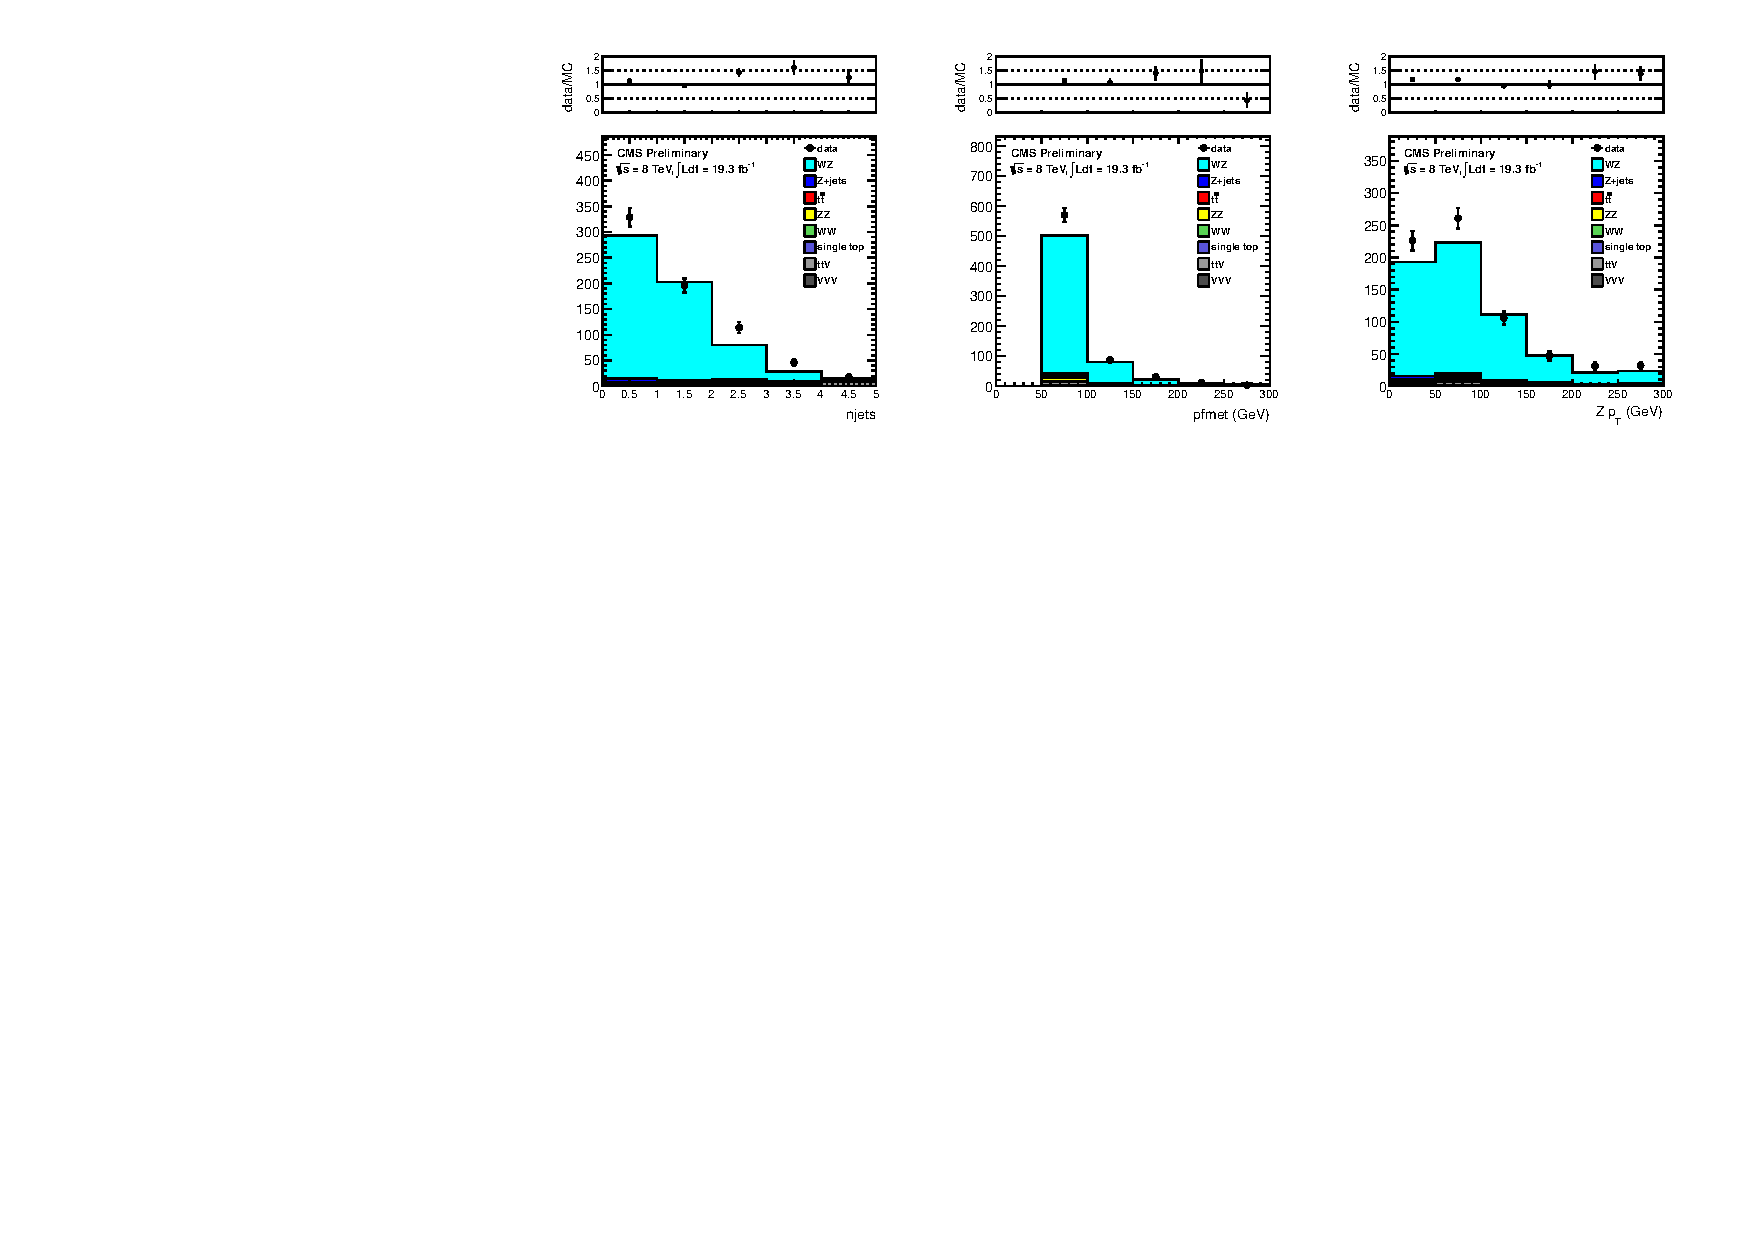
\includegraphics[width=1\linewidth]{plots/WZ_19fb.pdf}
\caption{\label{fig:wz}\protect 
Data vs. MC comparisons for the WZ selection discussed in the text for \lumi. 
The number of jets, missing transverse energy, and Z boson transverse momentum are displayed.
}
\begin{comment}
Loading babies at       : ../output/V00-02-00
Using selection         : (((((((leptype==0 && (ee==1 || isdata==0))||(leptype==1 && (mm==1 || isdata==0)))||(leptype==2 && (em==1||me==1||isdata==0)))&&(csc==0 && hbhe==1 && hcallaser==1 && ecaltp==1 && trkfail==1 && eebadsc==1 && hbhenew==1))&&(lep1.pt()>20.0 && lep2.pt()>20.0))&&(nlep==3 && lep3.pt()>20.0))&&(pfmet>50))&&(dilmass>81 && dilmass<101)
Using weight            : weight * 19.3 * trgeff * vtxweight
Plotting var njets flavor sf
compareDataMC : apply trigeff 1
MC yield VVV 7.73
MC yield ttV 18.95
MC yield single top 0.51
MC yield WW 0.09
MC yield ZZ 12.38
MC yield WZ 562.71
MC yield ttbar 9.18
SCALING ZJETS BY 111/946
MC yield zjets 8.85
MC total yield 620.39
data yield 703
Plotting var pfmet flavor sf
compareDataMC : apply trigeff 1
MC yield VVV 7.73
MC yield ttV 18.95
MC yield single top 0.51
MC yield WW 0.09
MC yield ZZ 12.38
MC yield WZ 562.72
MC yield ttbar 9.18
SCALING ZJETS BY 111/946
MC yield zjets 8.85
MC total yield 620.40
data yield 703
Plotting var dileppt flavor sf
compareDataMC : apply trigeff 1
MC yield VVV 7.73
MC yield ttV 18.95
MC yield single top 0.51
MC yield WW 0.09
MC yield ZZ 12.38
MC yield WZ 562.71
MC yield ttbar 9.18
SCALING ZJETS BY 111/946
MC yield zjets 8.85
MC total yield 620.38
data yield 703
\end{comment}

\end{center}
\end{figure}

\clearpage

\subsubsection{ZZ Validation Studies}
\label{sec:bkg_zz}

A pure ZZ sample can be selected in data with the requirements:

\begin{itemize}
\item Exactly 4 $p_T>20$~GeV leptons passing analysis identication and isolation requirements,
\item 2 of the 4 leptons must fall in the $Z$ window 81-101 GeV.
\end{itemize}

The data and MC yields passing the above selection are in Table~\ref{tab:zz}. 
In this ZZ-dominated sample we observe good agreement between the data yield and the MC prediction.
After requiring 2 jets (corresponding to the requirement in the analysis selection), we observe 14 events
in data and the MC predicts $13.2\pm0.2$ events. Due to the limited statistical precision we assign an uncertainty
of 50\% on the ZZ yield.

\begin{table}[htb]
\begin{center}
\caption{\label{tab:zz} Data and Monte Carlo yields for the ZZ preselection. }
\begin{tabular}{lccccc}

%Loading babies at       : ../output/V00-02-00
%Using selection         : ((((((leptype==0 && (ee==1 || isdata==0))||(leptype==1 && (mm==1 || isdata==0)))||(leptype==2 && (em==1||me==1||isdata==0)))&&(csc==0 && hbhe==1 && hcallaser==1 && ecaltp==1 && trkfail==1 && eebadsc==1 && hbhenew==1))&&(lep1.pt()>20.0 && lep2.pt()>20.0))&&(nlep==4 && lep3.pt()>20.0 && lep4.pt()>20.0))&&(dilmass>81 && dilmass<101)
%Using weight            : weight * 19.3 * trgeff * vtxweight

\hline
\hline
         Sample   &             ee   &       $\mu\mu$   &         e$\mu$   &          total  \\
\hline
%SCALING ZZ BY 1.92
             ZZ   & 52.7 $\pm$ 0.2   & 73.3 $\pm$ 0.2   &  3.4 $\pm$ 0.0   &129.4 $\pm$ 0.3  \\
             WZ   &  0.1 $\pm$ 0.0   &  0.1 $\pm$ 0.0   &  0.0 $\pm$ 0.0   &  0.3 $\pm$ 0.1  \\
%SCALING ZJETS BY 111/946
         \zjets   &  0.0 $\pm$ 0.0   &  0.0 $\pm$ 0.0   &  0.0 $\pm$ 0.0   &  0.0 $\pm$ 0.0  \\
         \ttbar   &  0.0 $\pm$ 0.0   &  0.0 $\pm$ 0.0   &  0.0 $\pm$ 0.0   &  0.0 $\pm$ 0.0  \\
             WW   &  0.0 $\pm$ 0.0   &  0.0 $\pm$ 0.0   &  0.0 $\pm$ 0.0   &  0.0 $\pm$ 0.0  \\
     single top   &  0.0 $\pm$ 0.0   &  0.0 $\pm$ 0.0   &  0.0 $\pm$ 0.0   &  0.0 $\pm$ 0.0  \\
            ttV   &  1.3 $\pm$ 0.2   &  1.4 $\pm$ 0.2   &  0.3 $\pm$ 0.1   &  3.0 $\pm$ 0.2  \\
            VVV   &  0.6 $\pm$ 0.1   &  0.8 $\pm$ 0.1   &  0.0 $\pm$ 0.0   &  1.4 $\pm$ 0.1  \\
\hline
      tot SM MC   & 54.7 $\pm$ 0.3   & 75.6 $\pm$ 0.3   &  3.8 $\pm$ 0.1   &134.1 $\pm$ 0.4  \\
\hline
           data   &             56   &             80   &              5   &            141  \\
\hline
\hline

\end{tabular}
\end{center}
\end{table}

\begin{figure}[tbh]
\begin{center}
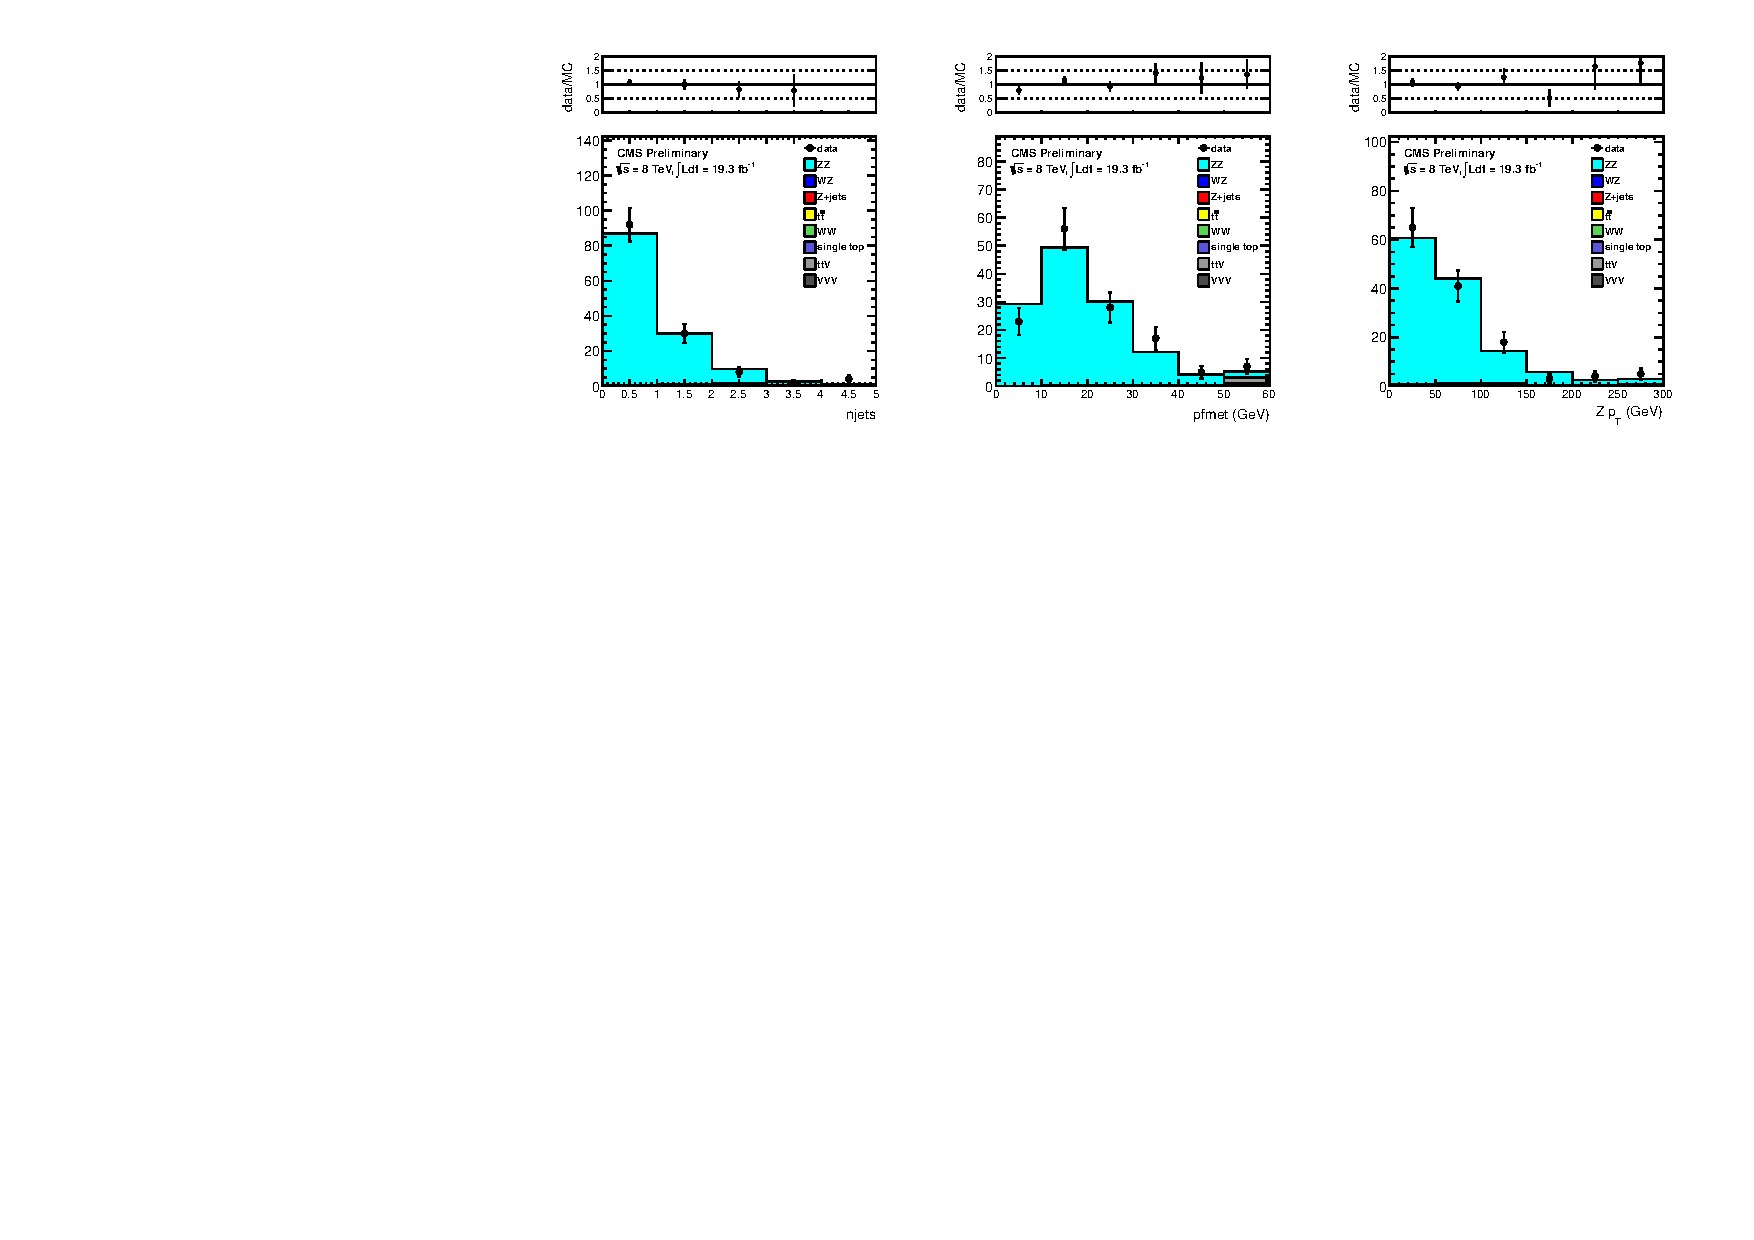
\includegraphics[width=1\linewidth]{plots/ZZ_19fb.pdf}
\caption{\label{fig:zz}\protect 
Data vs. MC comparisons for the ZZ selection discussed in the text for \lumi.
The number of jets, missing transverse energy, and Z boson transverse momentum are displayed.
}
\end{center}
\end{figure}

\begin{comment}
Loading babies at       : ../output/V00-02-00
Using selection         : ((((((leptype==0 && (ee==1 || isdata==0))||(leptype==1 && (mm==1 || isdata==0)))||(leptype==2 && (em==1||me==1||isdata==0)))&&(csc==0 && hbhe==1 && hcallaser==1 && ecaltp==1 && trkfail==1 && eebadsc==1 && hbhenew==1))&&(lep1.pt()>20.0 && lep2.pt()>20.0))&&(nlep==4 && lep3.pt()>20.0 && lep4.pt()>20.0))&&(dilmass>81 && dilmass<101)
Using weight            : weight * 19.3 * trgeff * vtxweight
Plotting var njets flavor sf
compareDataMC : apply trigeff 1

MC yield VVV 1.40
MC yield ttV 2.64
MC yield single top 0.00
MC yield WW 0.00
MC yield ttbar 0.00
SCALING ZJETS BY 111/946
MC yield zjets 0.00
MC yield WZ 0.27
SCALING ZJETS BY 1.92
MC yield ZZ 125.99
MC total yield 130.31
data yield 136
Plotting var pfmet flavor sf
compareDataMC : apply trigeff 1
MC yield VVV 1.40
MC yield ttV 2.64
MC yield single top 0.00
MC yield WW 0.00
MC yield ttbar 0.00
SCALING ZJETS BY 111/946
MC yield zjets 0.00
MC yield WZ 0.27
SCALING ZJETS BY 1.92
MC yield ZZ 126.00
MC total yield 130.32
data yield 136
Plotting var dileppt flavor sf
compareDataMC : apply trigeff 1
MC yield VVV 1.40
MC yield ttV 2.64
MC yield single top 0.00
MC yield WW 0.00
MC yield ttbar 0.00
SCALING ZJETS BY 111/946
MC yield zjets 0.00
MC yield WZ 0.27
SCALING ZJETS BY 1.92
MC yield ZZ 126.00
MC total yield 130.33
data yield 136
\end{comment}



%\subsection{Estimating the Rare SM Backgrounds with MC}
%\label{sec:bkg_raresm}

%{\bf TODO: list samples, yields in preselection region, and show \MET\ distribution}
